O serviço LDAP v3 do barramento de serviços ERLANGMS
refere-se a implementação protocolo
Lightweight Directory Access Protocol, ou LDAP,
um protocolo de aplicação aberto, livre de fornecedor e 
padrão de indústria que pode ser utilizado para oferecer
um "logon único" onde uma senha para um usuário é
compartilhada entre muitos serviços.

O barramento ERLANGMS foi desenvolvido 
com o intuíto de facilitar a modernização e a integração de 
sistemas por meio de uma abordagem orientada a serviços,
através do qual, serviços podem ser implementados e
disponibilizados aos usuários. Entre 
os serviços disponíveis, destaca-se
o serviço de autenticação de usuários LDAP v3.

Este capítulo aborda alguns conceitos que são
necessários para que o leitor possa obter um entendimento geral 
da arquitetura do barramento de serviços em tempo de execução.


\section{Software do barramento de serviços (ems-bus)}

O software do barramento denominado ems-bus 
tem a função de interligar os clientes (tipicamente os front-ends) 
aos serviços que contém as regras de negócios da organização (como o logon do usuário). 
Quando alguém faz uma requisição para um serviço, é o software do barramento 
que intermedia o envio e o recebimento das mensagens, sendo que o cliente
só precisa saber o endereço do barramento e o formato das mensagens utilizadas (ou protocolo). A 
Figura \ref{fig:roteamento_mensagens} mostra o esquema típico de
roteamento de mensagens do principal protocolo do barramento, o HTTP/REST. 
Convém salientar que este esquema é em tudo semelhante
ao protocolo LDAP v3 também.

\begin{figure}[htb]
\centering
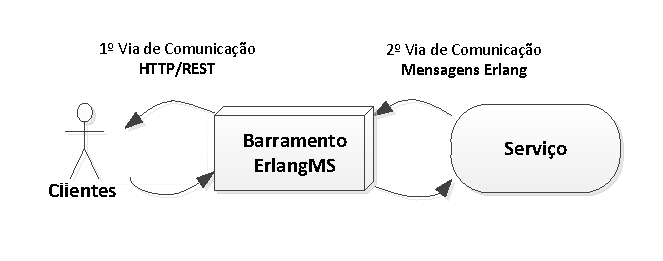
\includegraphics[scale=1.2]{/img/arquitetura/roteamento_mensagens.pdf}
\caption{Esquema do roteamento das mensagens da arquitetura.}
\label{fig:roteamento_mensagens}
\end{figure}
\FloatBarrier


\section{Catálogo de serviços}

Representa um componente chave da arquitetura do barramento de serviços pois permite
dar visibilidade aos serviços que serão disponibilizados aos clientes. É no catálogo
que são descritos e registrados (como um contrato) todas as informações sobre os serviços
que o cliente poderá consumir, por exemplo. A Figura~\ref{fig:catalogo_processo} exibe 
o contrato de serviço no catálogo 
de serviços do barramento para o LDAP v3.


\lstset{
        basicstyle=\footnotesize,
        numbers=left,
        numberstyle=\footnotesize,
        tabsize=2,
        numbers=none,
        rulesepcolor=\color{blue}}
\renewcommand{\lstlistingname}{Código}             
\begin{lstlisting}[caption=Contrato de serviço para o LDAP v3., label=fig:catalogo_processo] 
{
	"name": "ems_ldap_server",
	"comment": "LDAP service for client integration to the SCA database",
	"owner": "emsbus",
	"version": "1.0.0",
	"service" : "ems_ldap_server:start",
	"url": "/emsbus/ems_ldap_server",
	"type": "KERNEL",
	"lang" : "erlang",
	"tcp_listen_address" : ["0.0.0.0"],
	"tcp_allowed_address" : ["*.*.*.*"],
	"tcp_port": 2389,
	"datasource" : {
		"type" : "sqlserver",
		"connection" : "string conection",
		"primary_key" : "PesCodigoPessoa",
		"timeout" : 3000,
		"max_pool_size" : 10
	},	
	"ldap_admin" : "cn=admin,dc=unb,dc=br",
	"ldap_password_admin" : "xxxxxxxxx",
}
\end{lstlisting}


\section{Módulo Back-end}

O back-end é a implementação dos serviços. Tipicamente
os serviços são implementados na linguagem Java no CPD/UnB
mas podem ser desenvolvidos também em Erlang ou qualquer outra linguagem que possua 
o SDK do barramento de serviços. 


\section{Módulo Front-end}

O front-end é consumidor do serviço e o responsável por coletar os dados de entrada do usuário
e realizar as chamadas para os serviços por meio do barramento de serviços.
Em relação ao serviço LDAP, pode-se citar como exemplos de front-end, 
o Redmine, o SEI, o Joomla, entre outros.


\section{Servidor de Aplicação JBoss/Wildfly}

O servidor de aplicação JBoss/Wildfly é onde são publicados (deployment)
os projetos Java Web, que contém a implementação de serviços na linguagem Java. 
Podem existir várias instâncias desses servidores para
aumentar a escalabilidade dos serviços disponibilizados, 
sendo que o barramento despacha
as requisições dos clientes utilizando um algoritmo round-robin.

\section{Erlang Port Mapper Daemon}

É um processo que executa em 
segundo plano no sistema operacional em cada nó onde os serviços foram instalados e age 
como um servidor de nome para que o barramento consiga
enviar e receber mensagens dos processos de serviços.

